\documentclass[aspectratio=169]{../latex_main/tntbeamer}  % you can pass all options of the beamer class, e.g., 'handout' or 'aspectratio=43'
\usepackage{dsfont}
\usepackage{bm}
\usepackage[english]{babel}
\usepackage[T1]{fontenc}
%\usepackage[utf8]{inputenc}
\usepackage{graphicx}
\graphicspath{ {./figures/} }
\usepackage{algorithm}
\usepackage[ruled,vlined,algo2e,linesnumbered]{algorithm2e}
\usepackage{hyperref}
\usepackage{booktabs}
\usepackage{mathtools}

\usepackage{amsmath,amssymb}

\DeclareMathOperator*{\argmax}{arg\,max}
\DeclareMathOperator*{\argmin}{arg\,min}

\usepackage{amsbsy}
\newcommand{\vect}[1]{\bm{#1}}
%\newcommand{\vect}[1]{\boldsymbol{#1}}

\usepackage{pgfplots}
\pgfplotsset{compat=1.16}
\usepackage{tikz}
\usetikzlibrary{trees} 
\usetikzlibrary{shapes.geometric}
\usetikzlibrary{positioning,shapes,shadows,arrows,calc,mindmap}
\usetikzlibrary{positioning,fadings,through}
\usetikzlibrary{decorations.pathreplacing}
\usetikzlibrary{intersections}
\pgfdeclarelayer{background}
\pgfdeclarelayer{foreground}
\pgfsetlayers{background,main,foreground}
\tikzstyle{activity}=[rectangle, draw=black, rounded corners, text centered, text width=8em]
\tikzstyle{data}=[rectangle, draw=black, text centered, text width=8em]
\tikzstyle{myarrow}=[->, thick, draw=black]

% Define the layers to draw the diagram
\pgfdeclarelayer{background}
\pgfdeclarelayer{foreground}
\pgfsetlayers{background,main,foreground}

% Requires XeLaTeX or LuaLaTeX
%\usepackage{unicode-math}

\usepackage{fontspec}
%\setsansfont{Arial}
\setsansfont{RotisSansSerifStd}[ 
Path=../latex_main/fonts/,
Extension = .otf,
UprightFont = *-Regular,  % or *-Light
BoldFont = *-ExtraBold,  % or *-Bold
ItalicFont = *-Italic
]
\setmonofont{Cascadia Mono}[
Scale=0.8
]

\renewcommand{\ttdefault}{Cascadia Mono}

% scale factor adapted; mathrm font added (Benjamin Spitschan @TNT, 2021-06-01)
%\setmathfont[Scale=1.05]{Libertinus Math}
%\setmathrm[Scale=1.05]{Libertinus Math}

% other available math fonts are (not exhaustive)
% Latin Modern Math
% XITS Math
% Libertinus Math
% Asana Math
% Fira Math
% TeX Gyre Pagella Math
% TeX Gyre Bonum Math
% TeX Gyre Schola Math
% TeX Gyre Termes Math

% Literature References
\newcommand{\lit}[2]{\href{#2}{\footnotesize\color{black!60}[#1]}}

%%% Beamer Customization
%----------------------------------------------------------------------
% (Don't) Show sections in frame header. Options: 'sections', 'sections light', empty
\setbeamertemplate{headline}{empty}

% Add header logo for normal frames
\setheaderimage{
	% 
\includegraphics[height=\logoheight]{figures/TNT_darkv4.pdf}
	
\includegraphics[height=\logoheight]{../latex_main/figures/Leibniz-AI-Academy_Logo}
	% 
\includegraphics[height=\logoheight]{figures/logo_tntluh.pdf}
}

% Header logo for title page
\settitleheaderimage{
	% 
\includegraphics[height=\logoheight]{figures/TNT_darkv4.pdf}
	
\includegraphics[height=\logoheight]{../latex_main/figures/Leibniz-AI-Academy_Logo}
	% 
\includegraphics[height=\logoheight]{figures/logo_tntluh.pdf}
}

% Title page: tntdefault 
\setbeamertemplate{title page}[tntdefault]  % or luhstyle
% Add optional title image here
%\addtitlepageimagedefault{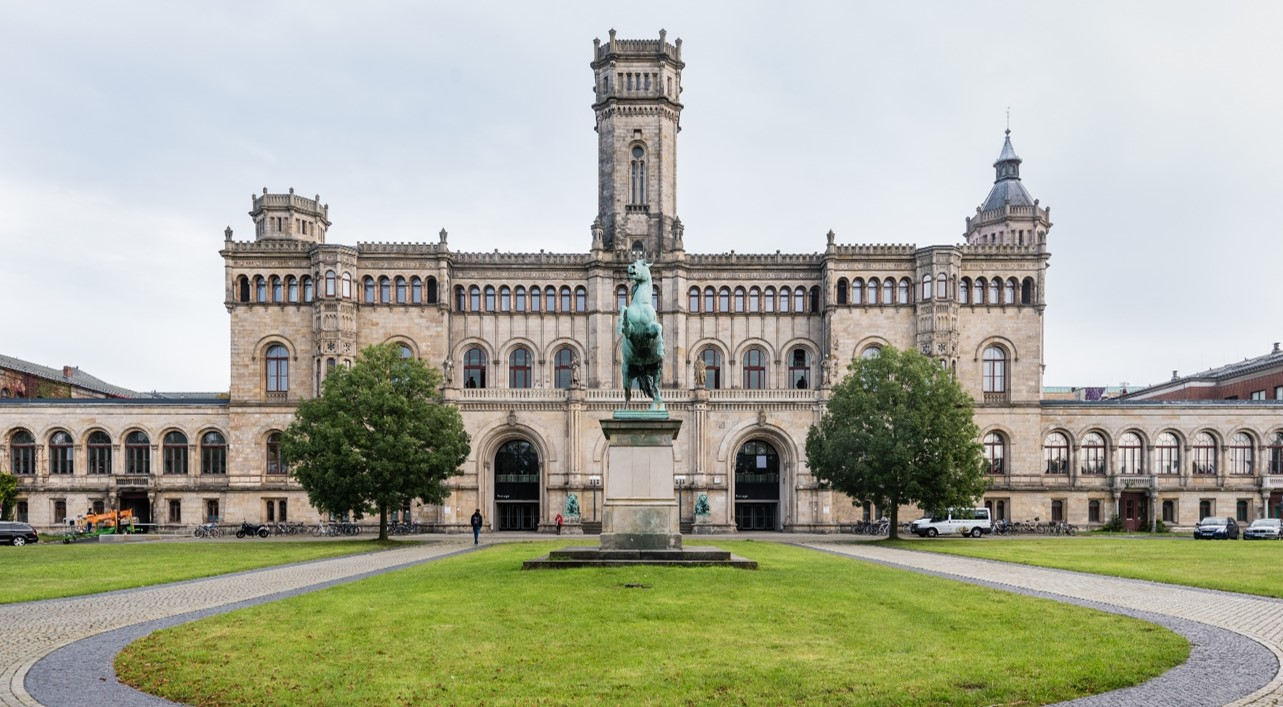
\includegraphics[width=0.65\textwidth]{figures/luh_default_presentation_title_image.jpg}}

% Title page: luhstyle
% \setbeamertemplate{title page}[luhstyle]
% % Add optional title image here
% \addtitlepageimage{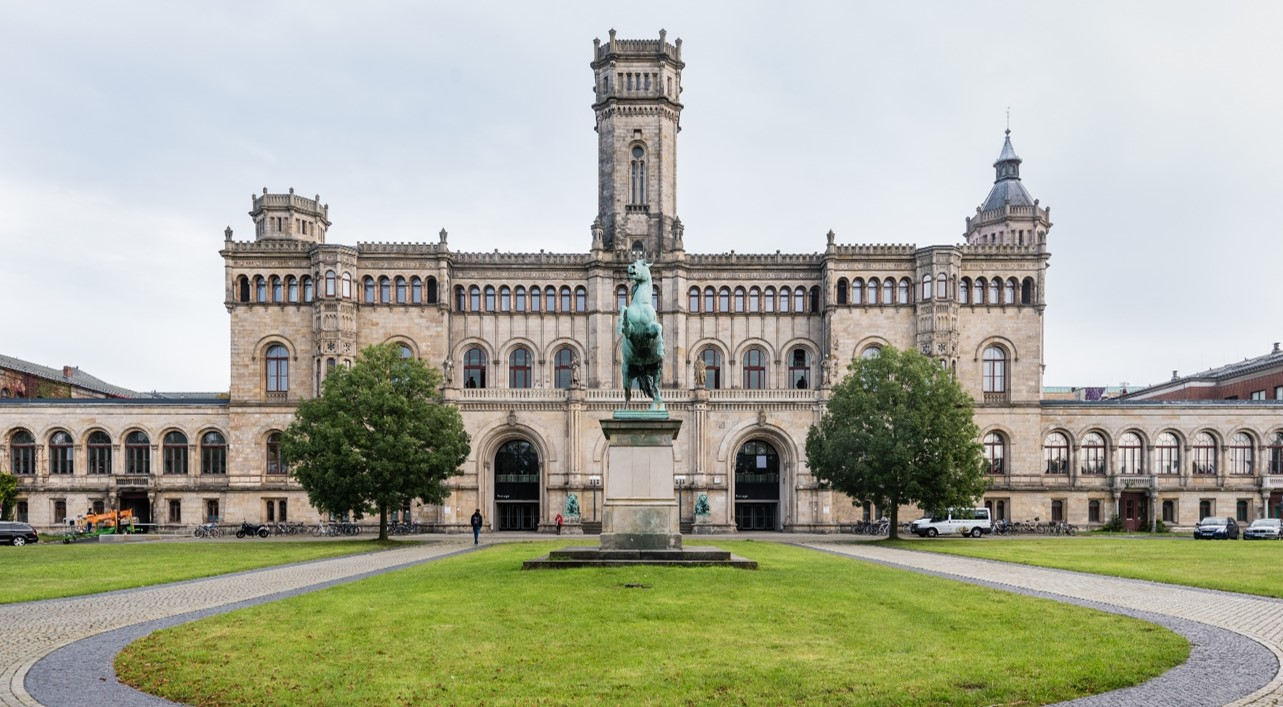
\includegraphics[width=0.75\textwidth]{figures/luh_default_presentation_title_image.jpg}}

\author[Abedjan \& Lindauer]{Ziawasch Abedjan \& \underline{Marius Lindauer}\\[1em]
	%
\includegraphics[height=\logoheight]{../latex_main/figures/luh_logo_rgb_0_80_155.pdf}\qquad
	
\includegraphics[height=\logoheight]{../latex_main/figures/DBIS_Kurzlogo.png}\qquad
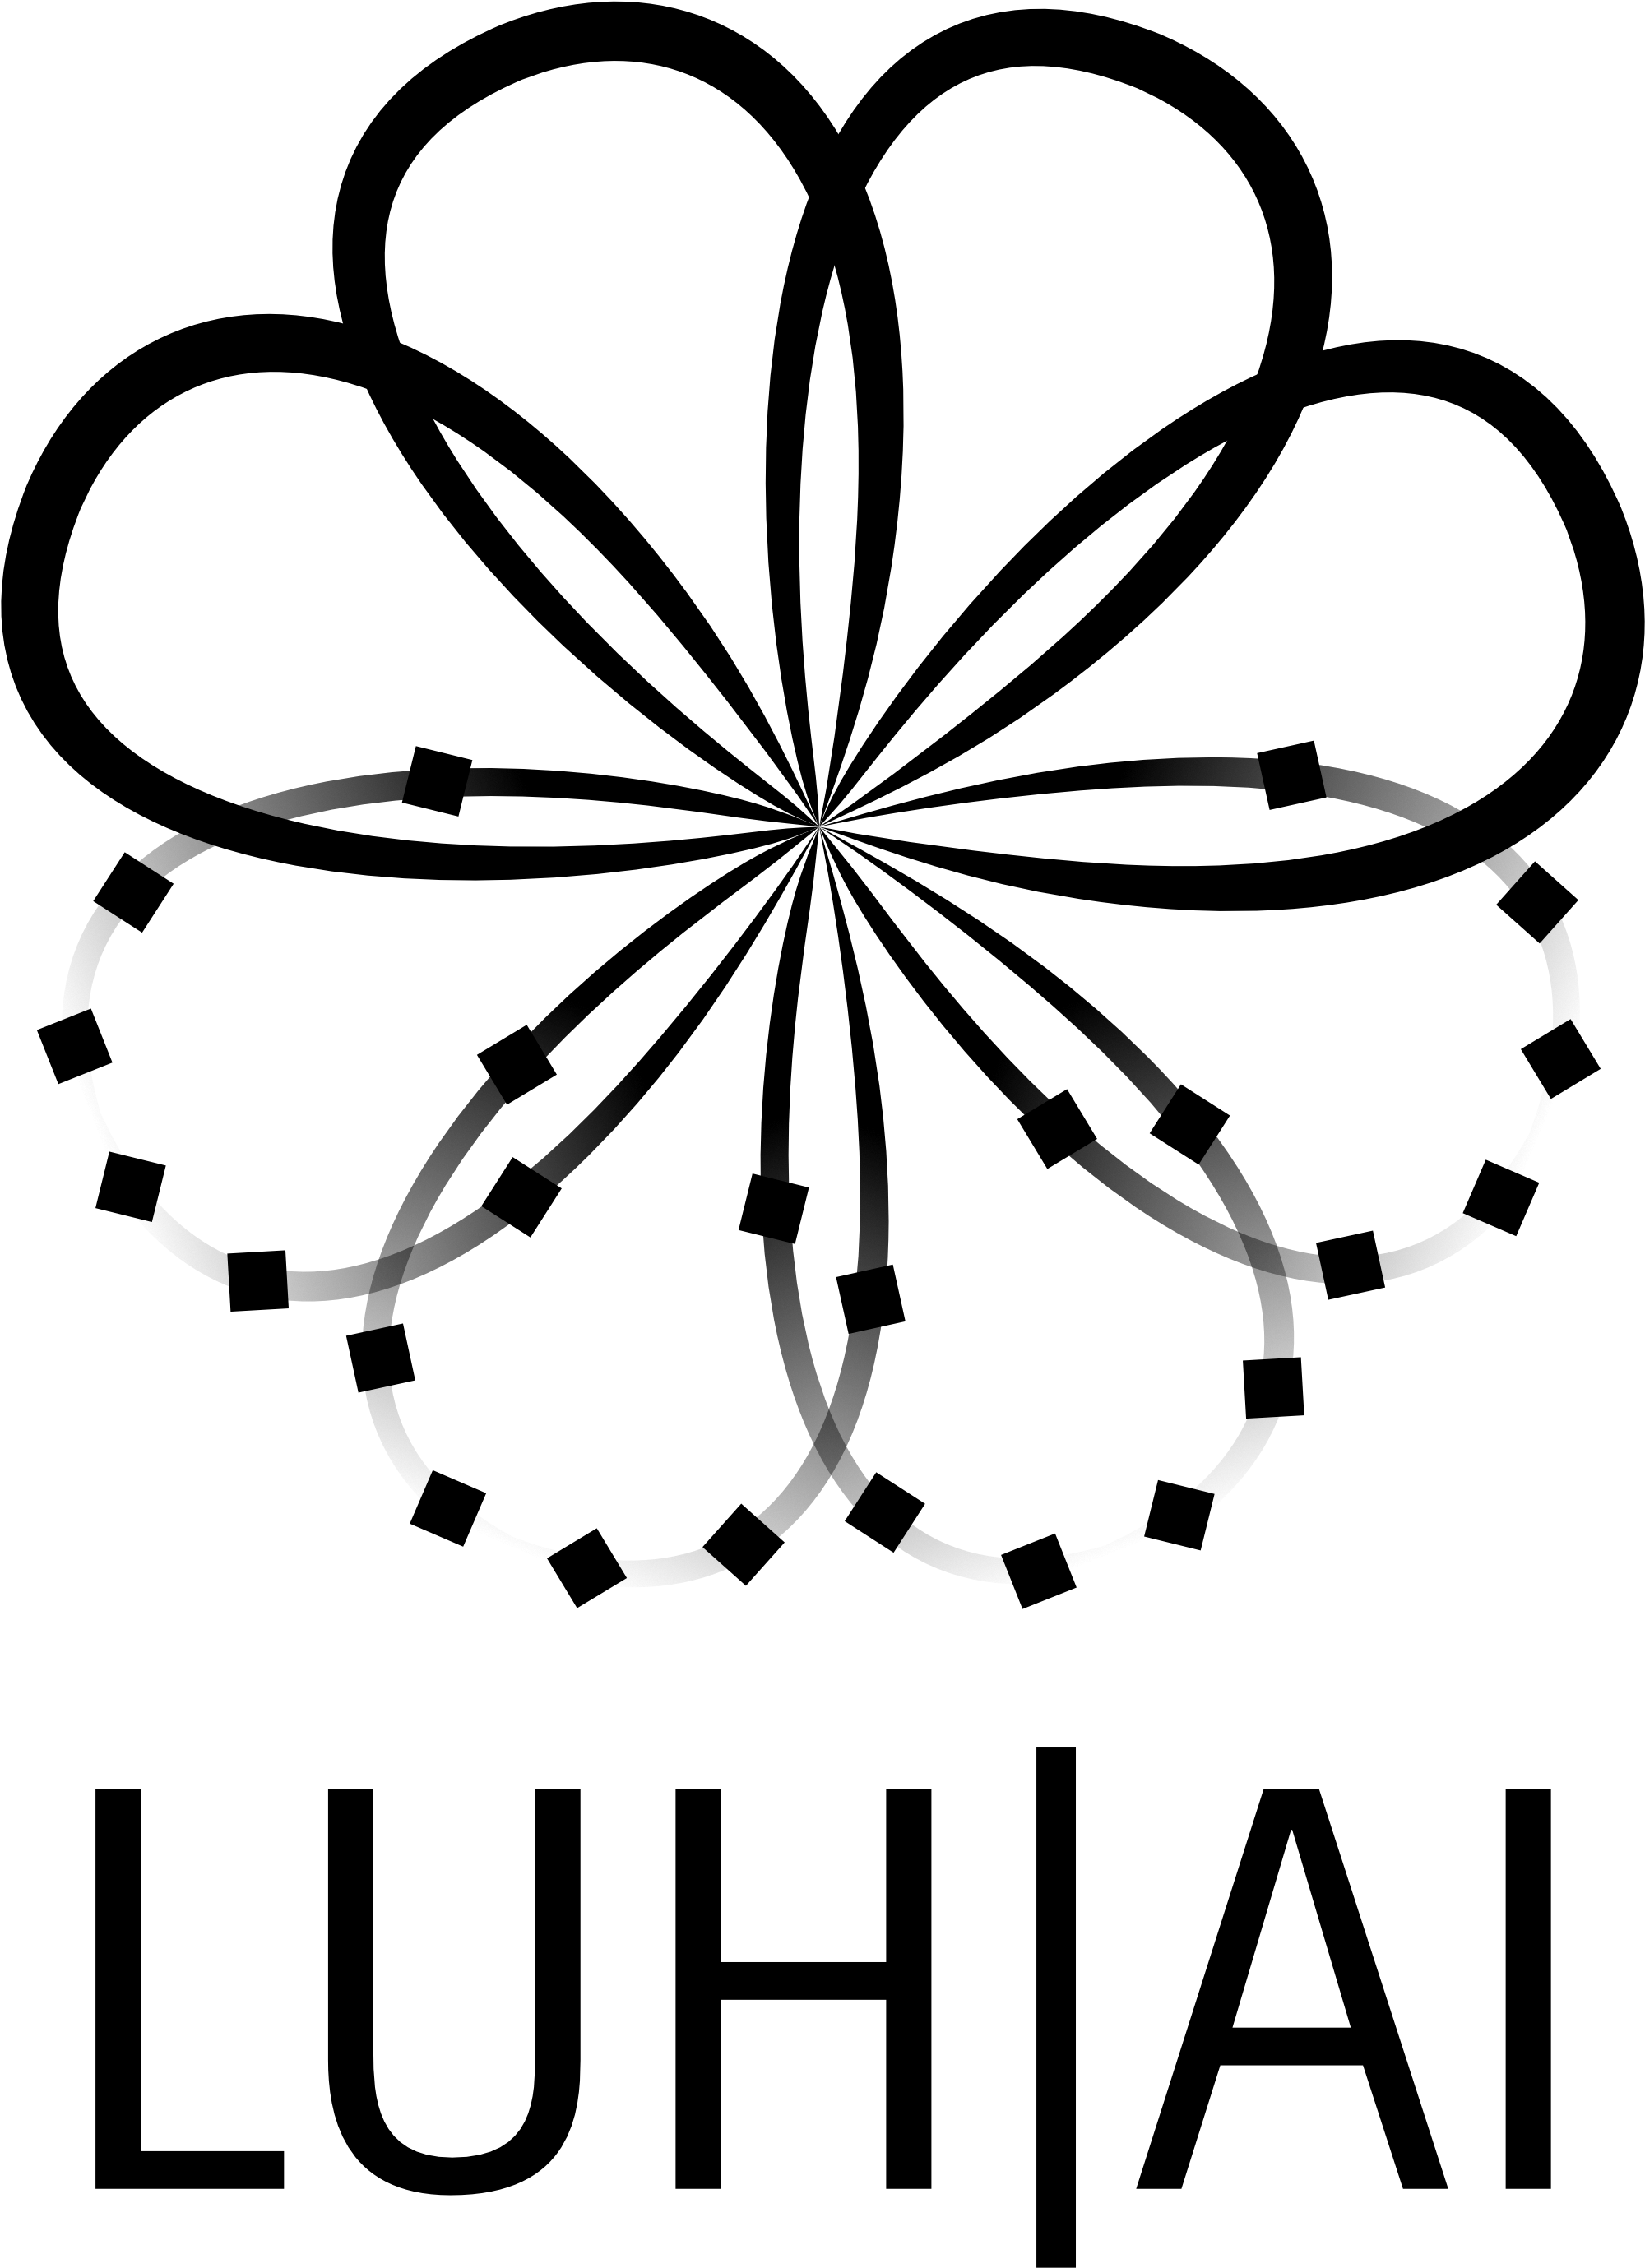
\includegraphics[height=\logoheight]{../latex_main/figures/logo_short_highres_black}\qquad

\includegraphics[height=\logoheight]{../latex_main/figures/Leibniz-AI-Academy_Logo}\qquad
%
\includegraphics[height=\logoheight]{../latex_main/figures/L3S.jpg}	
}
\date{\hspace{0.5em} {
\includegraphics[height=1.5em]{../latex_main/figures/Cc-by-nc-sa_icon.svg.png}}; extension of \href{https://ds100.org/fa21/}{[DS100]}
}


%%% Custom Packages
%----------------------------------------------------------------------
% Create dummy content
\usepackage{blindtext}

% Adds a frame with the current page layout. Just call \layout inside of a frame.
\usepackage{layout}


%%% Macros
%\renewcommand{\vec}[1]{\mathbf{#1}}
% \usepackage{bm}
%\let\vecb\bm

\title[Data Property: Structure]{DS: Data Cleaning}
\subtitle{Data Property: Structure}

\graphicspath{ {./figure/} }
%\institute{}


\begin{document}
	
	\maketitle

% Slide 9 - Key Data Properties
\begin{frame}[c]{Key Data Properties to Consider in EDA}
    \begin{itemize}
        \item \textbf{Structure} -- the “shape” of a data file.
        \item {Granularity} -- how fine/coarse is each datum.
        \item {Scope} -- how (in)complete is the data.
        \item {Temporality} -- how is the data situated in time.
        \item {Faithfulness} --how well does the data capture “reality”.
    \end{itemize}
\end{frame}

\begin{frame}[c]{Using Data?}

``If we just have a bunch of data sets in a repository, it is unlikely anyone will ever be able to find, let alone reuse, any of this data. With adequate metadata, there is some
hope, but even so, challenges will remain...''

\bigskip

\textit{[D. Agrawal, P. Bernstein, E. Bertino, S. Davidson, U. Dayal, M. Franklin, J. Gehrke, L. Haas, A. Halevy, J. Han, H. V. Jagadish, A. Labrinidis , S. Madden , Y. Papakonstantinou , J. M. Patel, R. Ramakrishnan , K. Ross, C. Shahabi , D. Suciu, S. Vaithyanathan , and J. Widom. Challenges and opportunities with Big Data. Technical report, Computing Community Consortium,
http://cra.org/ccc/docs/ init/bigdatawhitepaper.pdf, 2012.]}

\end{frame}

\begin{frame}[c]{Data Tables?}

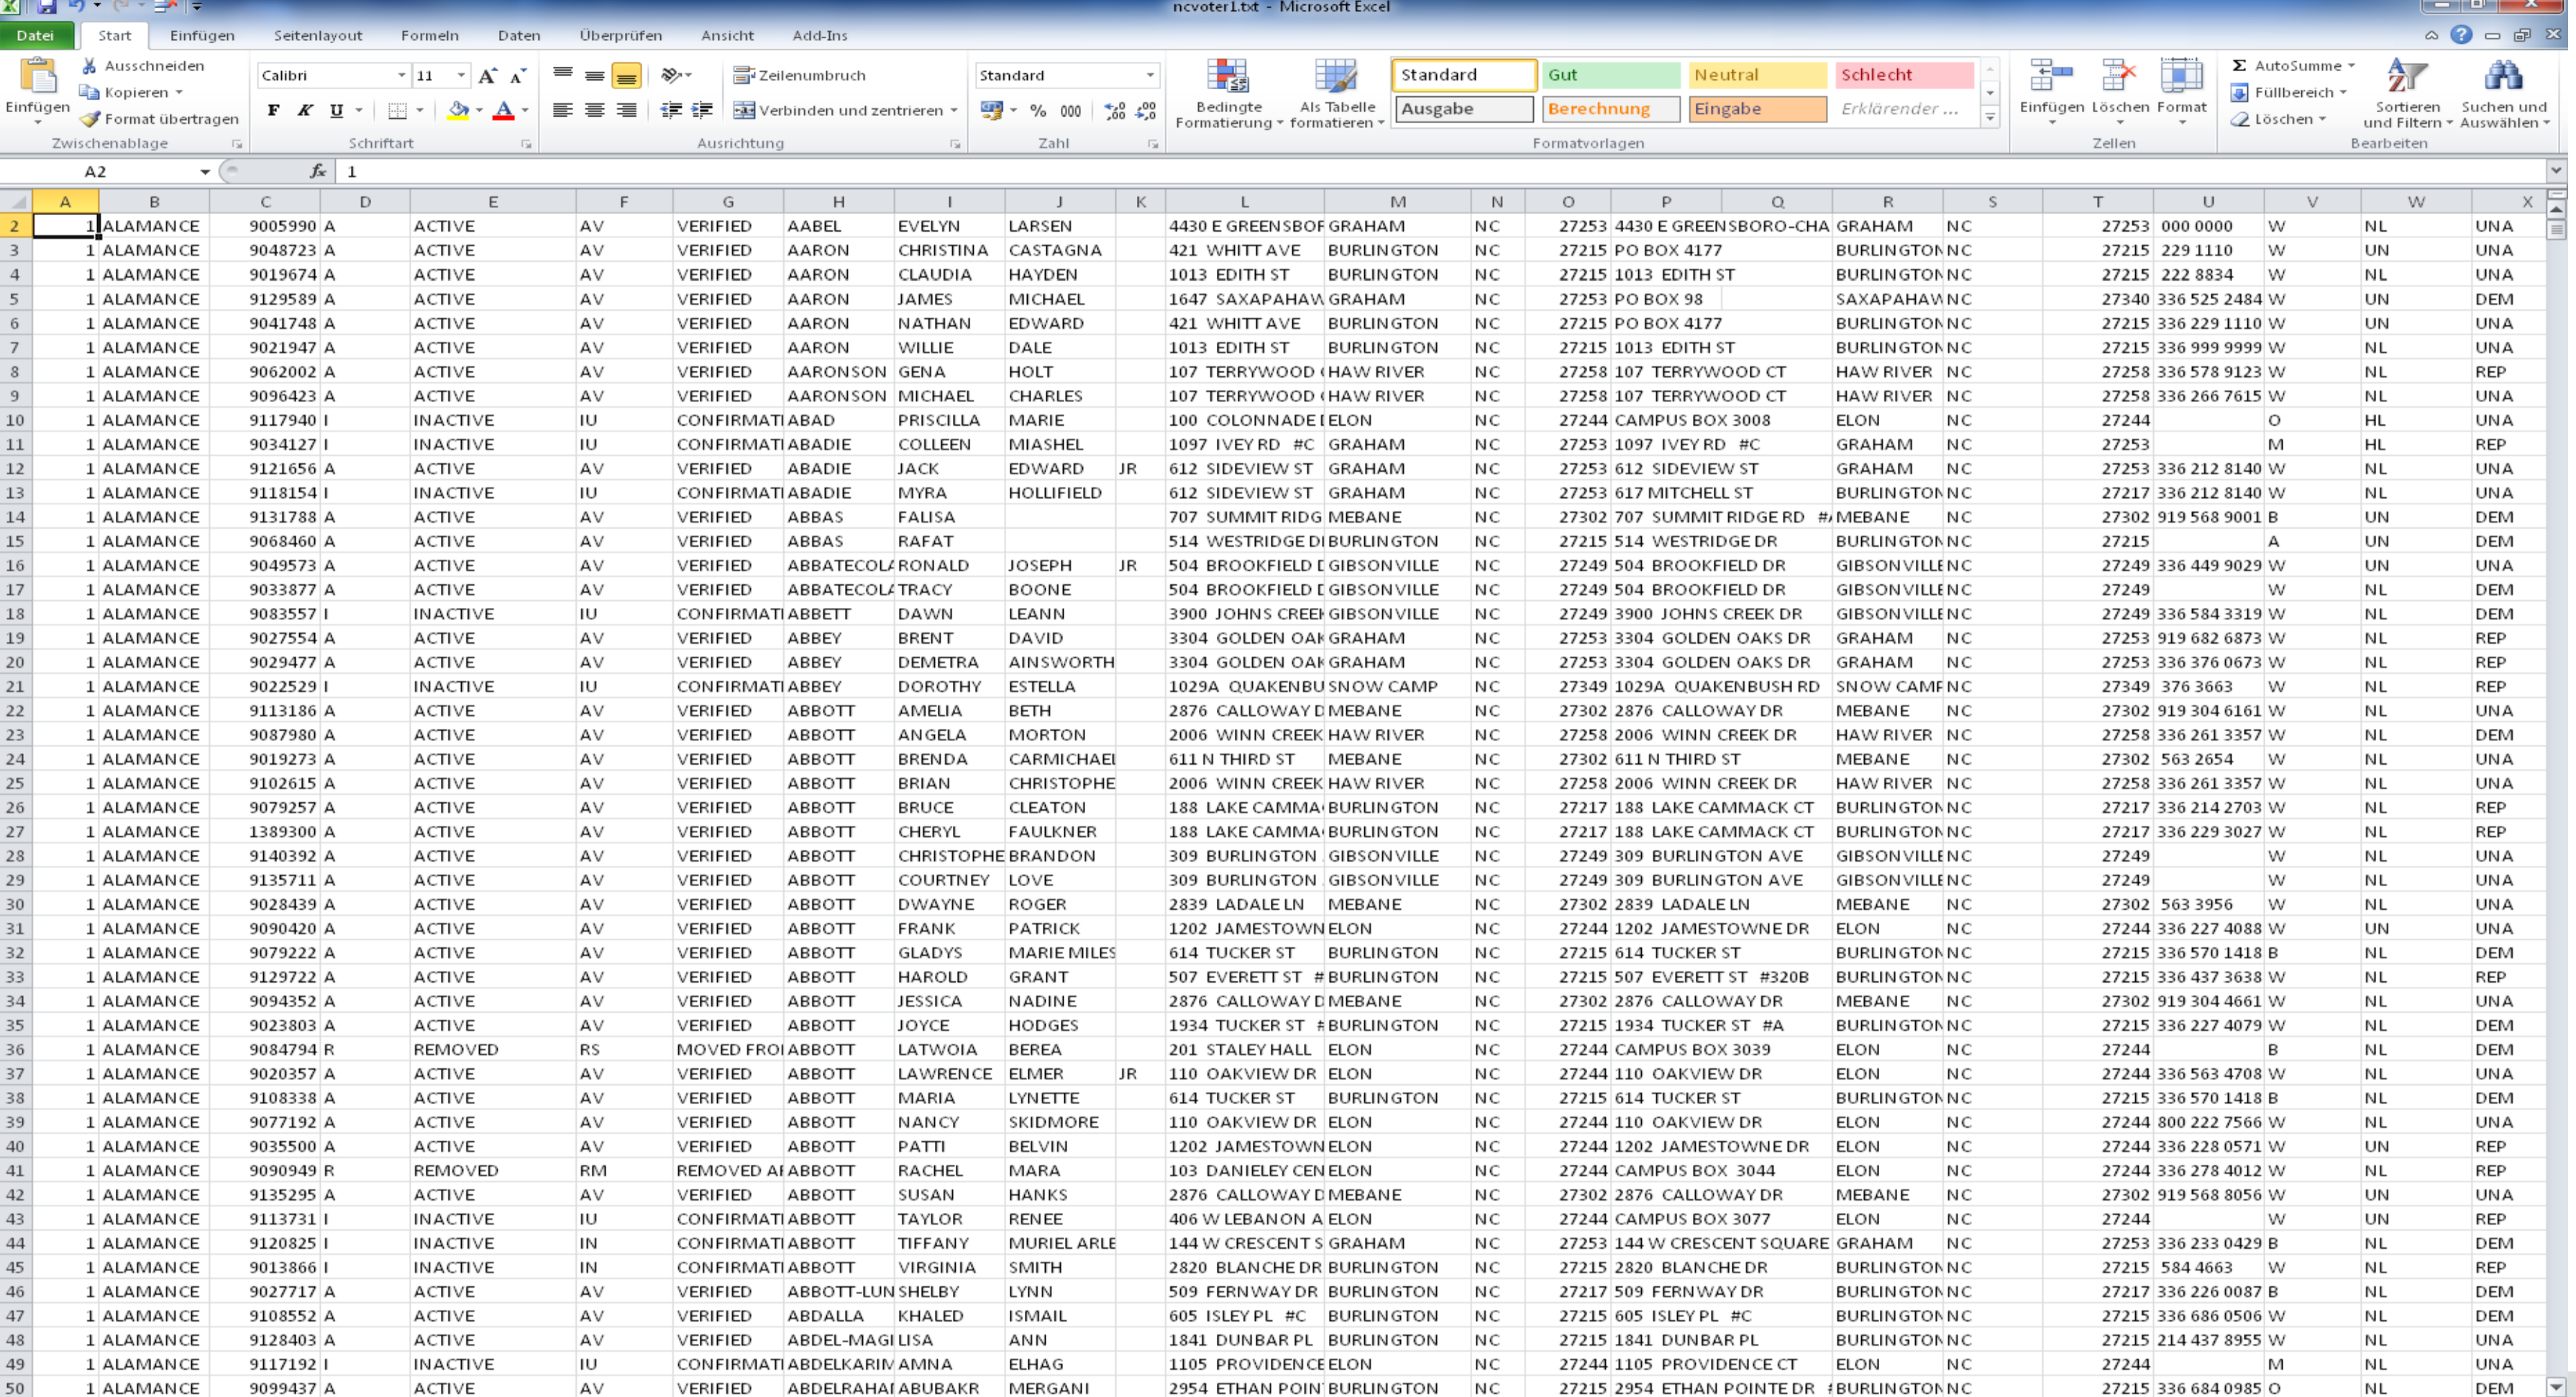
\includegraphics[width=1.0\textwidth]{bild6_excel}

\end{frame}

\begin{frame}[c]{Size of Data Tables?}

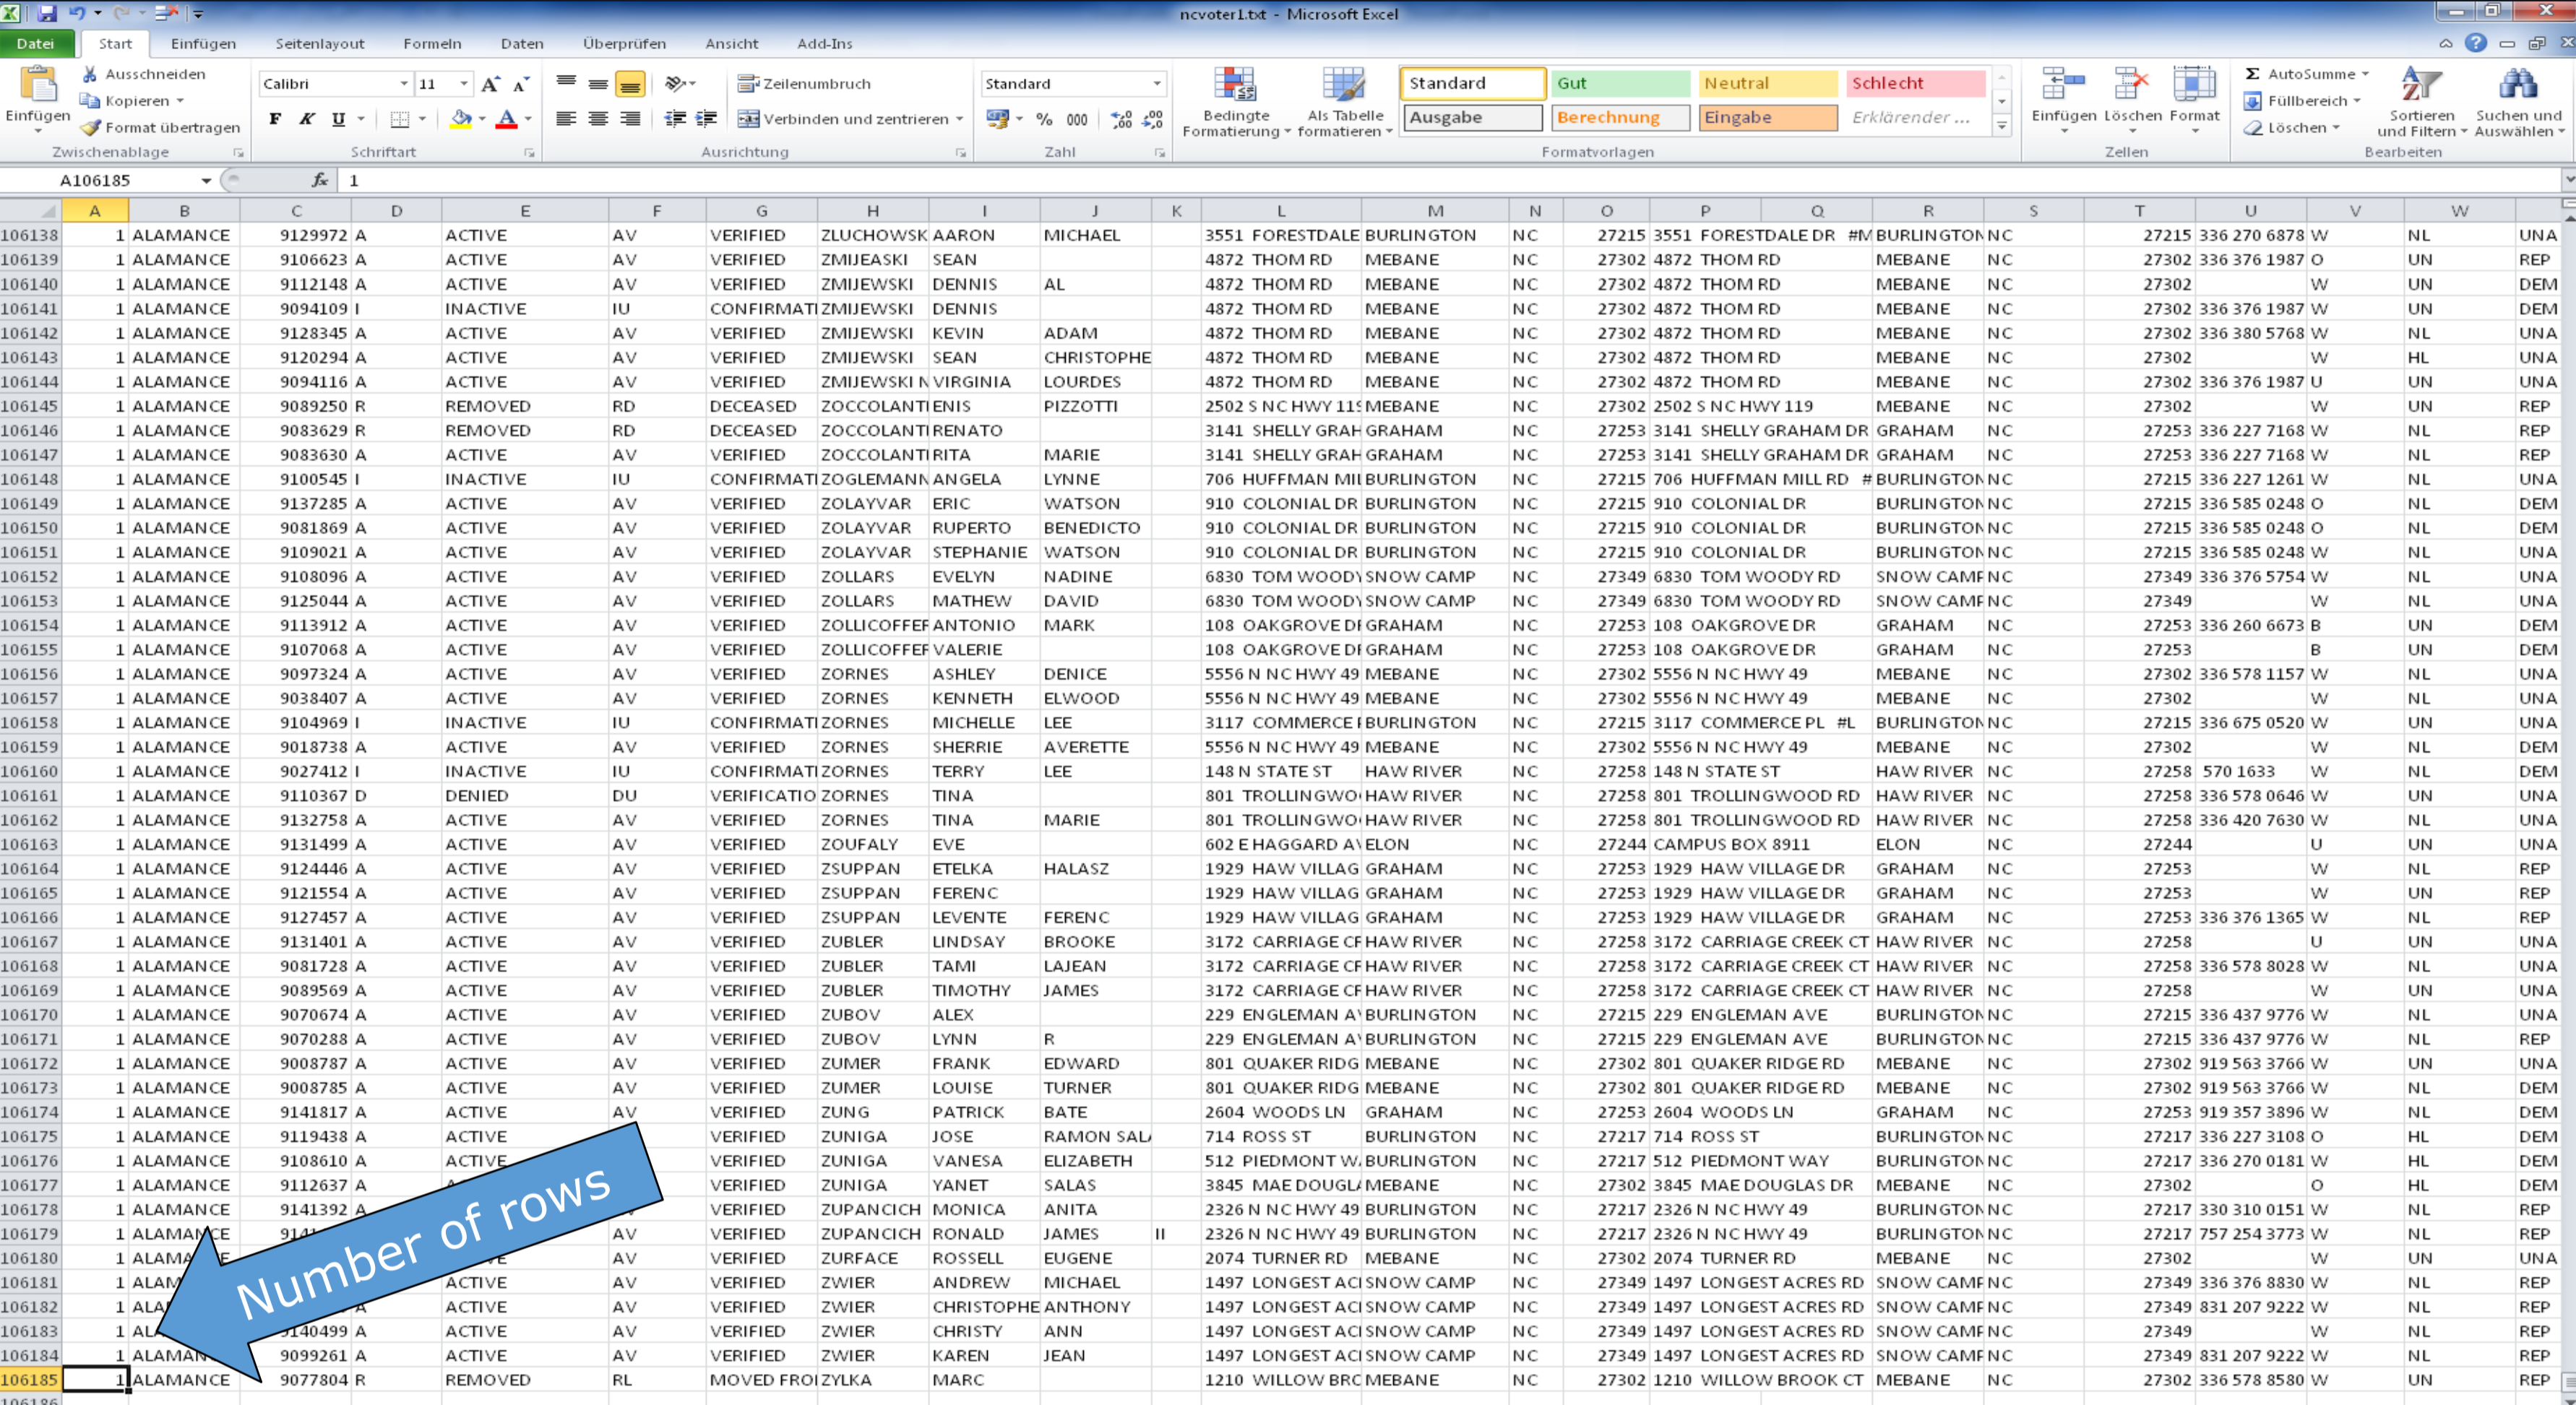
\includegraphics[width=0.8\textwidth]{bild7_rows}

\end{frame}


\begin{frame}[c]{Columns in Data Tables?}

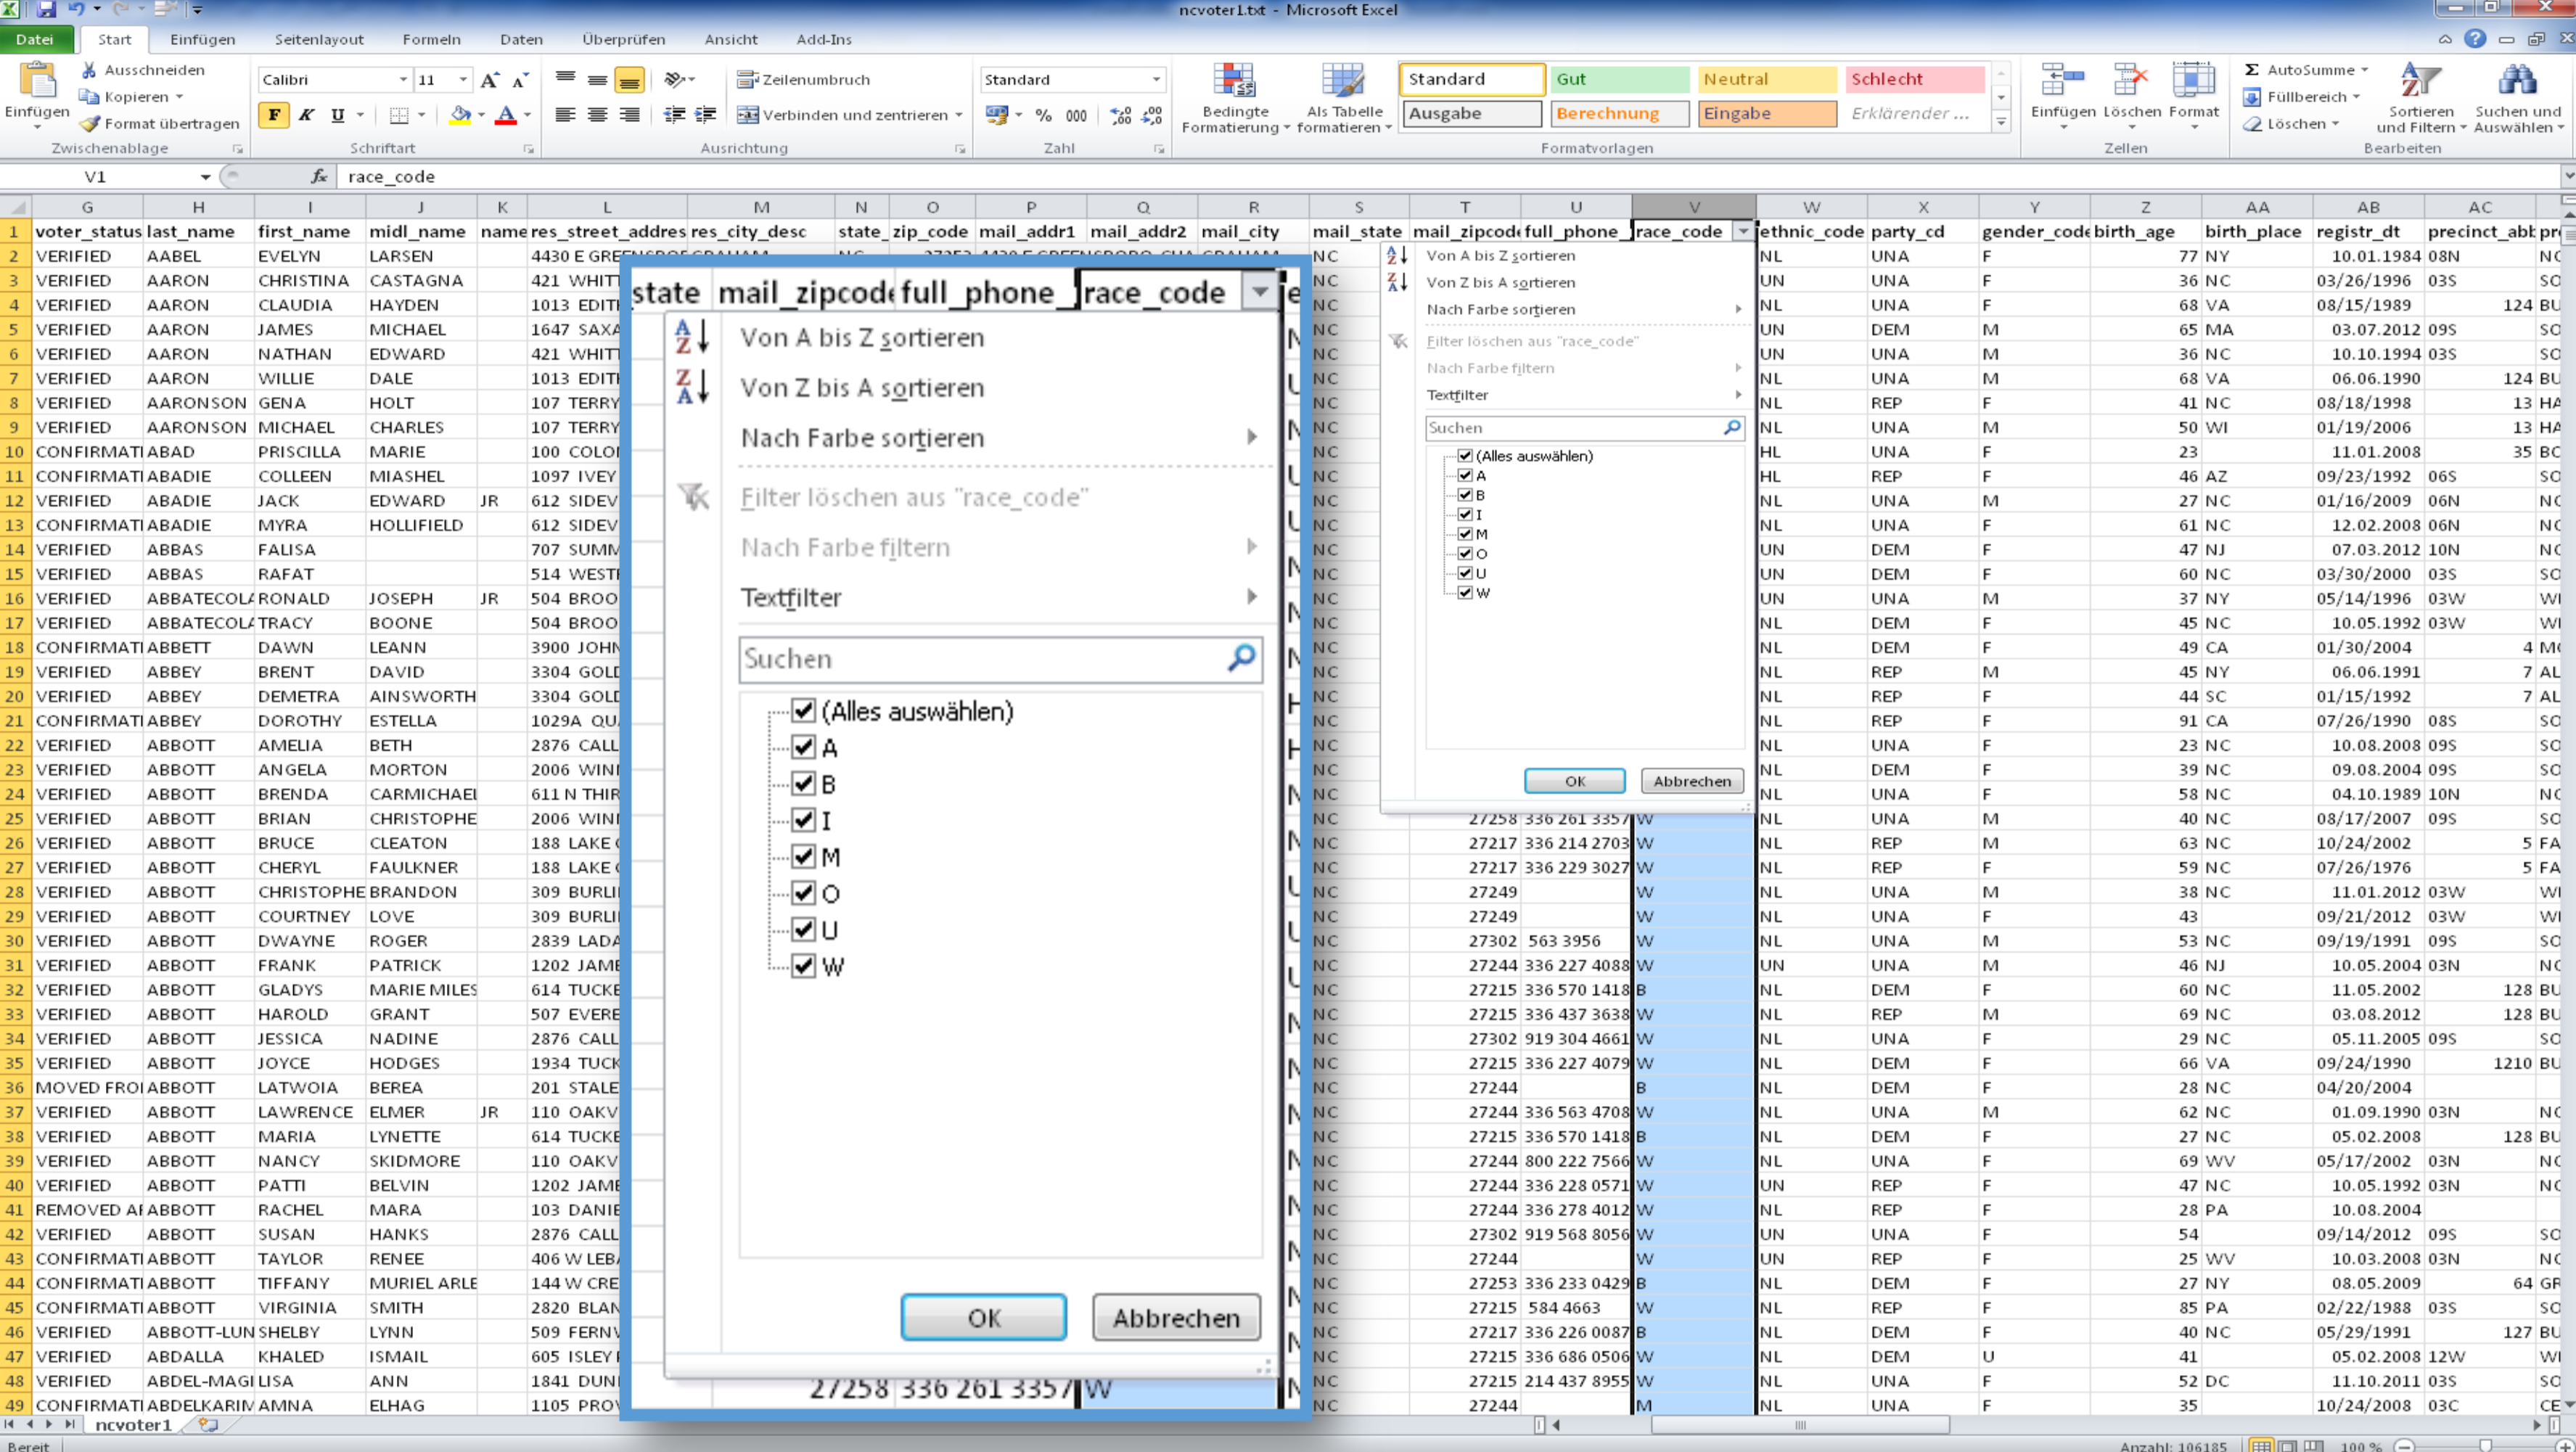
\includegraphics[width=1.0\textwidth]{bild8_race_code}

\end{frame}

\begin{frame}[c]{Many interesting question remain}

\begin{itemize}
    \item Many interesting questions remain What are possible keys and foreign keys?
    \begin{itemize}
        \item Phone
        \item firstname, lastname, street 
    \end{itemize}
    \item Are there any functional dependencies?
    \begin{itemize}
        \item zip -> city
        \item race -> voting behavior 
    \end{itemize}
    \item Which columns correlate?
    \begin{itemize}
        \item Date-of-Birth and first name 
        \item State and last name
    \end{itemize}
    \item What are frequent patterns in a column?
    \begin{itemize}
        \item ddddd
        \item dd aaaa St
    \end{itemize}

    \end{itemize}

\end{frame}

\begin{frame}[c]{Definition Data Profiling}

\begin{description}
    \item[Wikipedia] ``Data profiling is the process of examining the data available in an existing data source [...] and collecting statistics and information about that data.''
    \item[Ted Johnson] ``Data profiling refers to the activity of creating small but informative summaries of a database.''
    \item[Felix Neumann] Data profiling is the set of activities and processes to determine the metadata about a given dataset.
\end{description}

\end{frame}


% Slide 18 - Profiling Tasks
\begin{frame}[c]{Classification of Traditional Profiling Tasks}
    \centering
    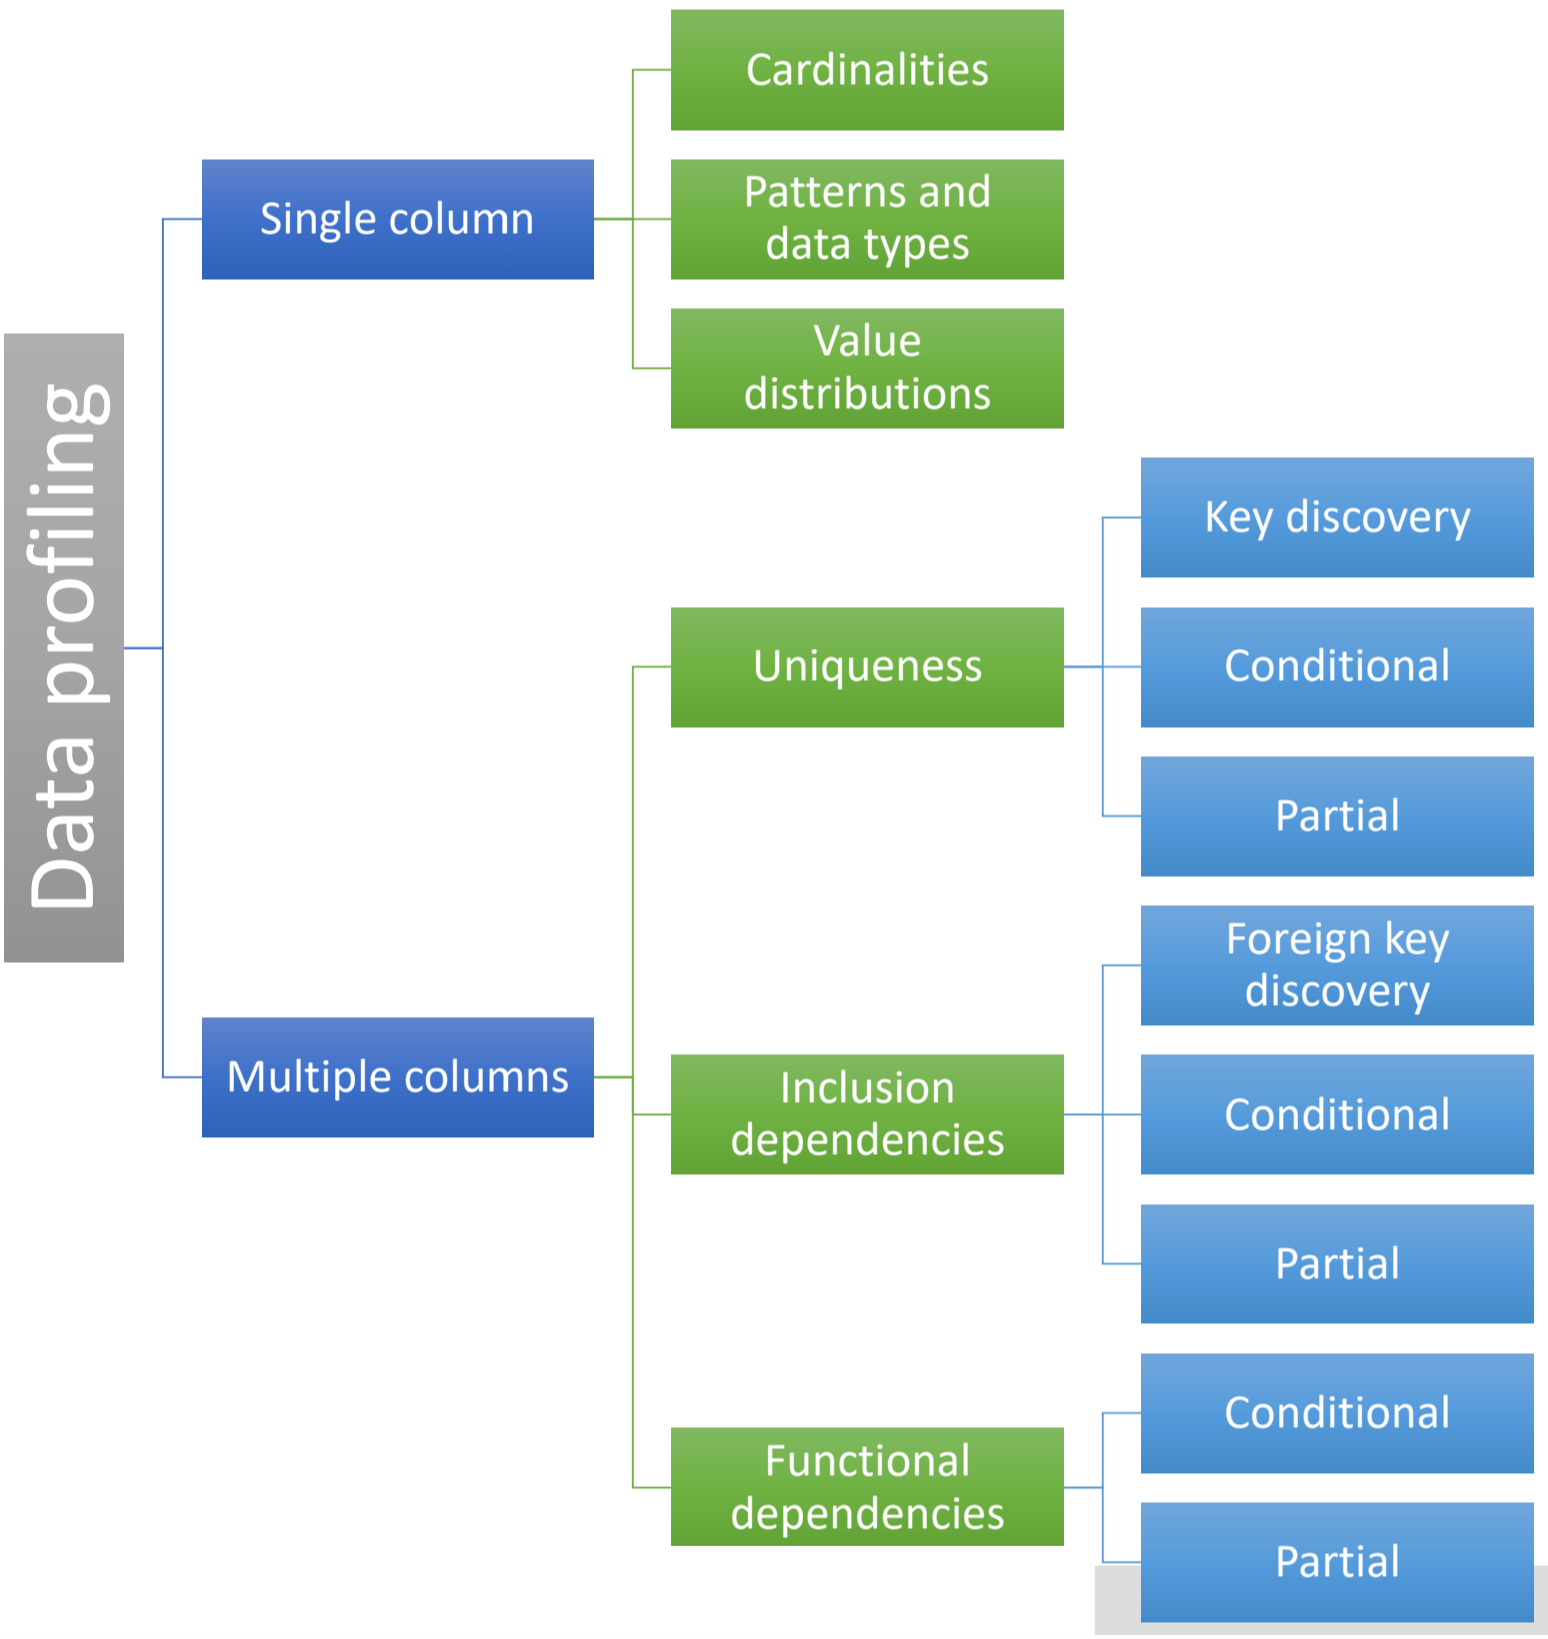
\includegraphics[width=.4\textwidth]{bild9_profiling}

    Abedjan, Golab, Naumann. Profiling Relationale Data: A Survey. VLDBJ 2015
\end{frame}

% Slide 19 - Rectangular Data
\begin{frame}[c]{Rectangular Data}
    \begin{itemize}
        \item We prefer rectangular data for data analysis (why?) 
        \item Rectangular structures are easy to manipulate and analyze 
        \item A big part of data preparation is about transforming data to be more rectangular
        \item Two types: \textbf{tables} (data-frames) and \textbf{matrices}.
        \begin{itemize}
            \item Tables: Named columns, different types.
            \item Matrices: Numeric data of same type; Manipulated using linear algebra
        \end{itemize}
    \end{itemize}
\end{frame}

% Slide 20 - Data Format
\begin{frame}[c]{}
    % \begin{itemize}
    %     \item TSV - Tab-separated values.
    %     \item CSV - Comma separated values.
    %     \item JSON - Nested data.
    % \end{itemize}
    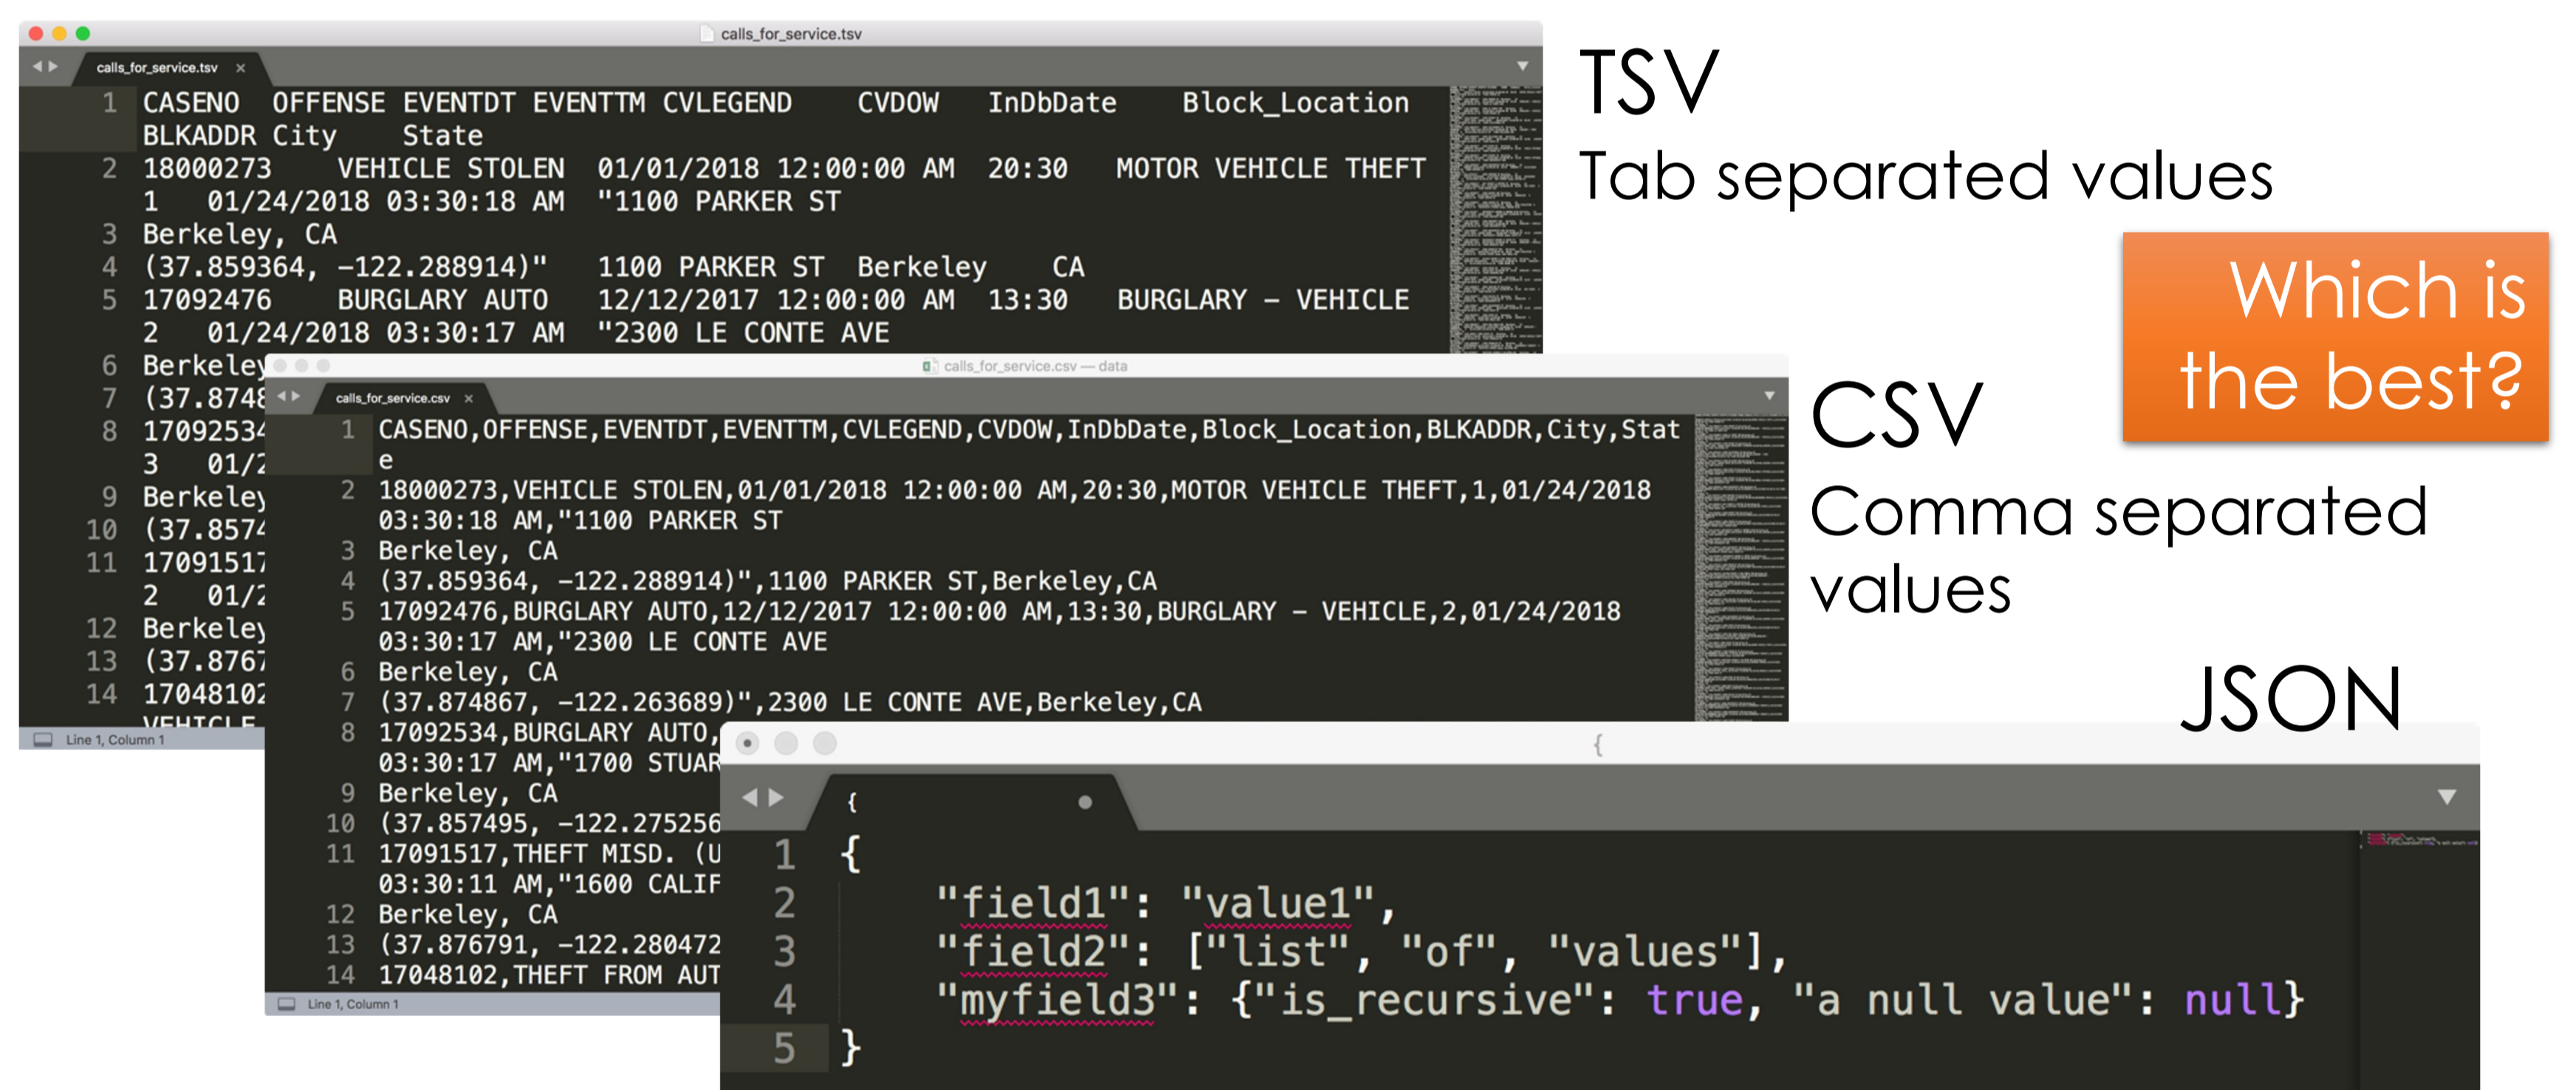
\includegraphics[width=1.0\textwidth]{bild10_file_formats}
\end{frame}



\begin{frame}[c]{Data Formats}
    \begin{itemize}
        \item Comma and Tab Separated Values Files
        \begin{itemize}
            \item Records delimited by newlines.
            \item Fields separated by commas or tabs.
            \item Issues: 
            \begin{itemize}
                \item commas, tabs inside records
                \item quoting
                \item missing headers
                \item several schemas
            \end{itemize}
        \end{itemize}
        \item JavaScript Object Notation (JSON)
        \begin{itemize}
            \item Format for nested data.
            \item Addresses some CSV/TSV issues.
            \item Issues: 
            \begin{itemize}
                \item each record can have different fields
                \item nesting means records can contain tables 
            \end{itemize}
        \end{itemize}
        \item other formats:
        \begin{itemize}
            \item XML
            \item arbitrary log data formats ...
        \end{itemize}
    \end{itemize}
\end{frame}


% Slide 25 - Structure Keys
\begin{frame}[c]{Structure: Keys}

\begin{columns}

\begin{column}{0.5\textwidth}

    \begin{itemize}
        \item Often data will reference other pieces of data
        \item Primary Key: the column or set of columns in a
table that determines the values of the remaining columns
        \item Foreign Key: References primary key in other tables.
        \item You will need to join across tables
    \end{itemize}
    
    \end{column}

    \begin{column}{0.5\textwidth}
    
        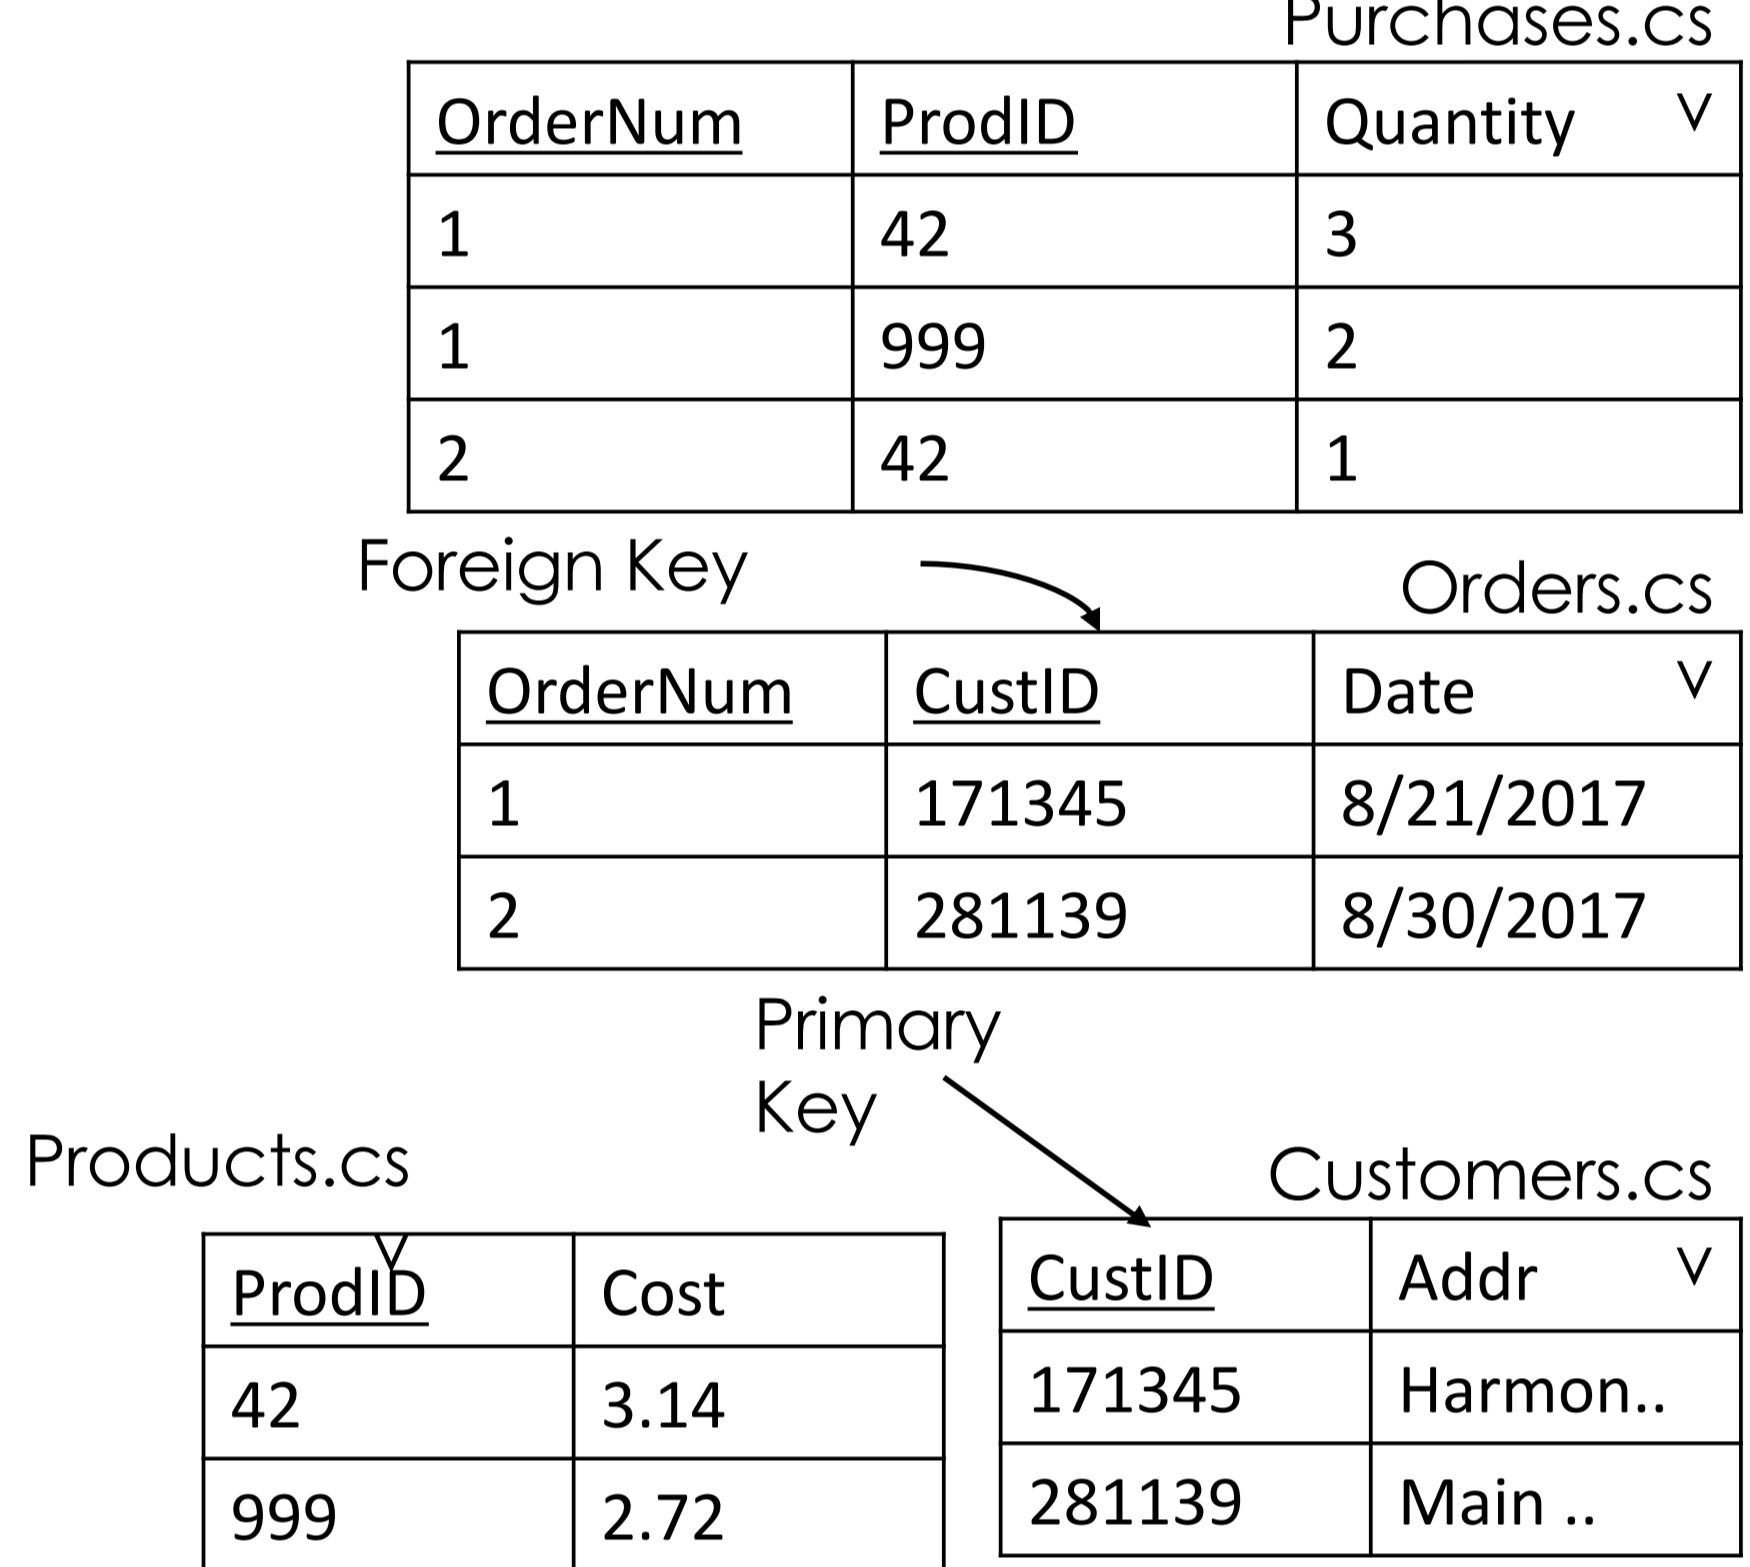
\includegraphics[width=.8\textwidth]{bild11_db}
            
    \end{column}

\end{columns}

\end{frame}

% Slide 27 - Types of Variables
\begin{frame}[c]{Types of Variables}

    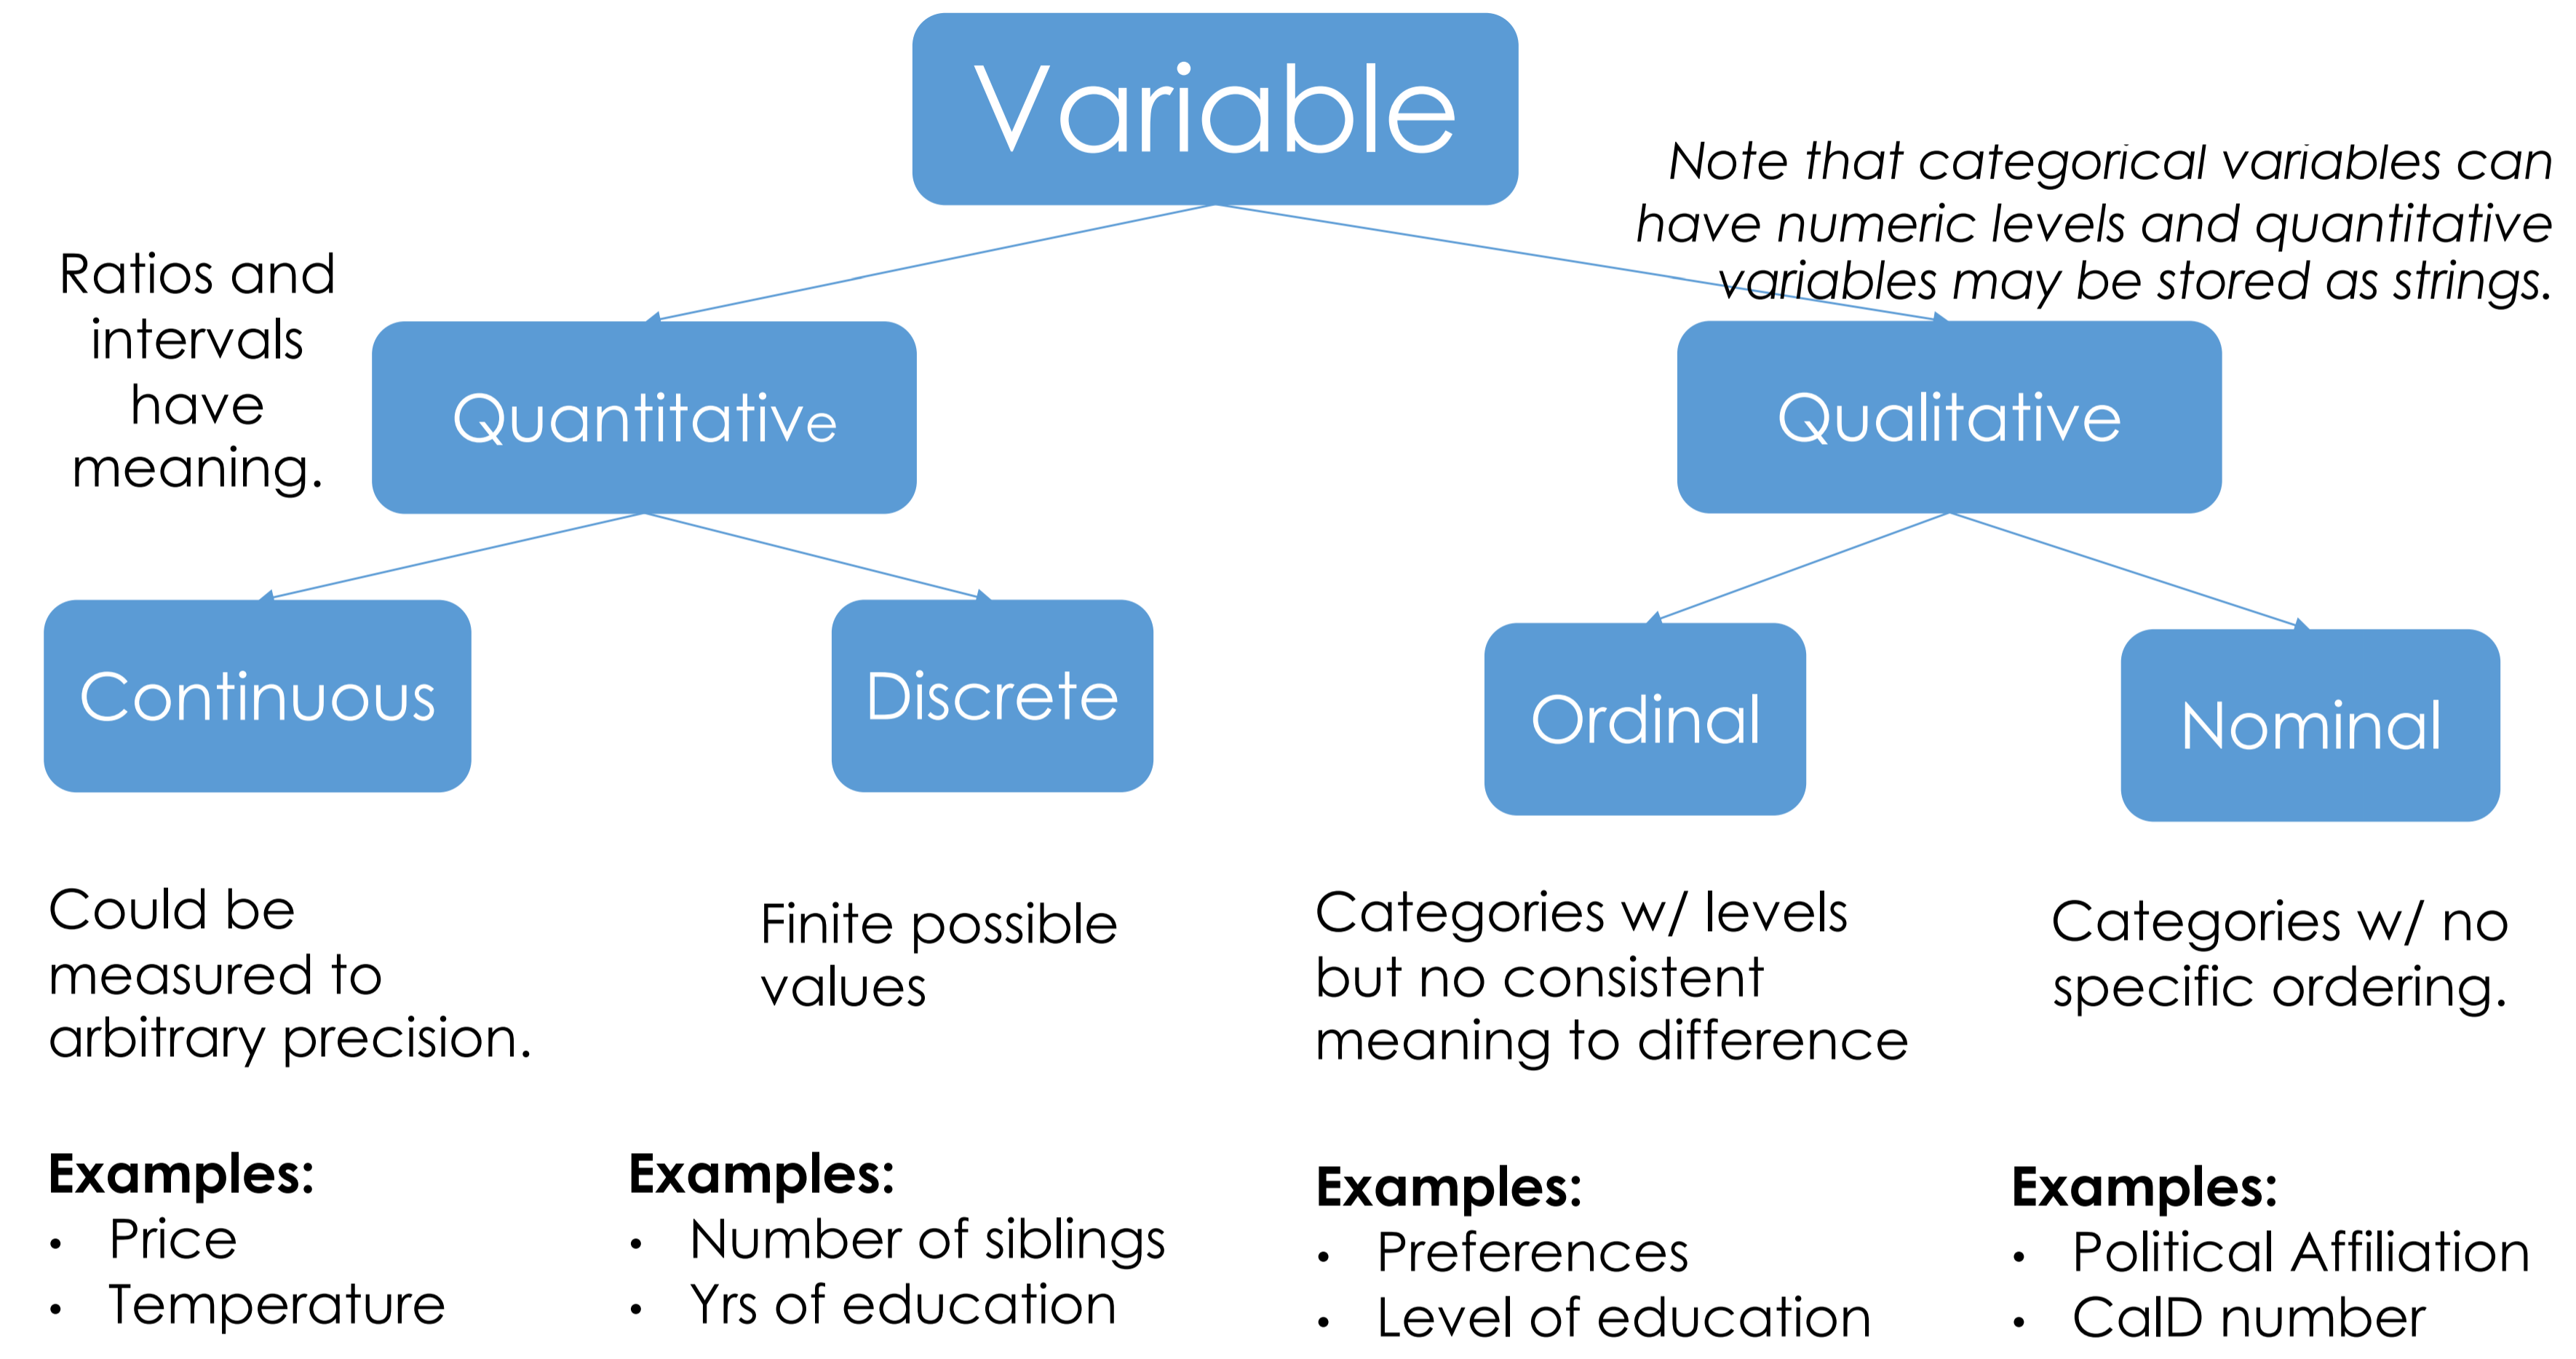
\includegraphics[width=.8\textwidth]{bild11_variable}
    
\end{frame}




\end{document}